\section{Theorie}

\subsection{Der ATLAS-Detektor}
Die Daten, die wir auswerten wollen, wurden im LHC am ATLAS-Detektor aufgenommen.
Um die Daten zu verstehen, ist es notwendig etwas darüber zu wissen, wie die Daten entstanden sind.
Daher schauen wir uns im folgenden den ATLAS-Detektor näher an.
Eine schematische Darstellung von diesem ist in Abb. \ref{ATLAS_schema_label} zu sehen.
\begin{figure}[ht]
	\centering
  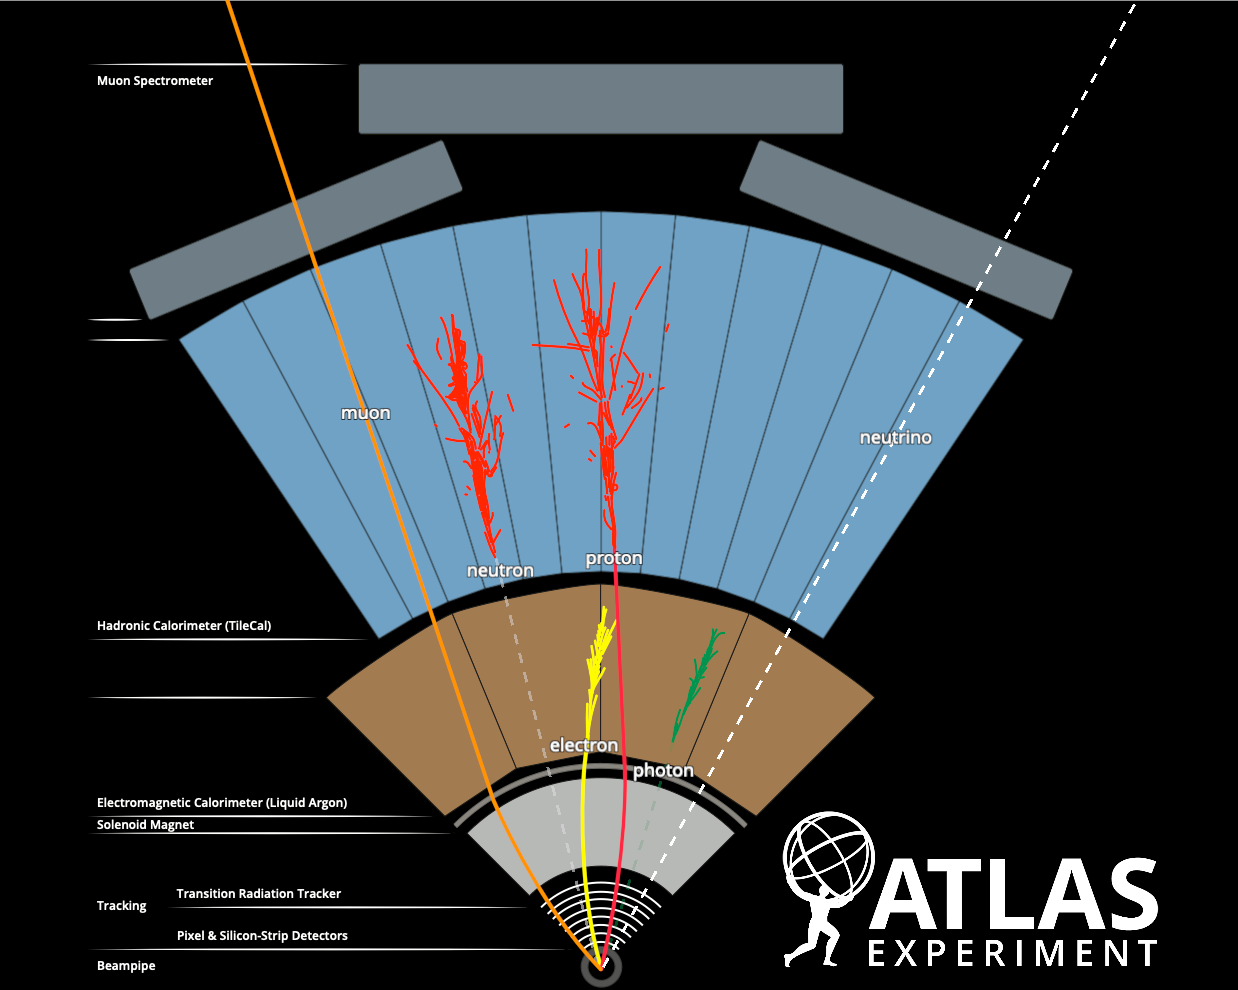
\includegraphics[width=0.95\textwidth]{../Pictures/ATLAS_Detector_Schematic_black_(PNG).png}
	\caption{Schematik ATLAS-Detektor im Querschnitt. \cite{ATLAS_schema}}
	\label{ATLAS_schema_label}
\end{figure}
Der Detektor besteht im wesentlichen aus vier Komponenten, von innen nach außen:
\begin{itemize}
  \item Ein Tracking-Detektor.
  \item Ein elektromagnetisches Kalorimeter.
  \item Ein hadronisches Kalorimeter.
  \item Ein Myon-Spektrometer.
\end{itemize}
Viele Teilchen die bei der Kollision von zwei Protonen entstehen können haben mittlere Lebensdauern von weniger als \SI{10e-10}{\second}.
Damit erreichen diese Teilchen den Detektor selbst so gut wie nie.
Man kann jedoch durch deren Zerfallsprodukte auf die Teilchen selbst schließen.
Im folgenden werden wir die Detektorkomponenten näher erläutern.

\subsubsection{Tracking-Detektoren}
Der Tracking-Detektor besteht aus mehreren Komponenten.
Diese haben die Aufgabe, die Trajektorie einiger Teilchen die bei den Proton-Protonkollisionen entstehen, aufzuzeichnen.
Die innerste Komponente stellt dabei ein Silizium-Pixeldetektor dar, der im Radialabstand von \SI{5}{\centi\meter} bis \SI{15}{\centi\meter} vom Protonenstrahl sitzt.
Er besitzt über 80 Millionen Pixel die parallel verarbeitet werden.
Mit dem Pixeldetektor wird der primäre Wechselwirkungspunkt rekonstruiert.
Außerdem werden sekundäre Vertices rekonstruiert, die beim Zerfall langlebiger Hadronen mit b-Quark-Inhalt entstehen können.
Die nächste Komponente ist ein Silizium-Halbleitertracker.
Dabei handelt es sich um Streifen, die ebenfalls präzise Spurpunkte liefern.
Darauf folgt ein Übergangsstrahlungsdetektor.
Hier sind gasgefüllte Driftkammern verbaut, in denen das Signal ionisierender Teilchen durch Übergangsstrahlung angereichert wird.
Als letzte Komponente dieses Detektorteils gibt es noch eine Reihe an Spulen.
Sie werden supraleitend betrieben, und halten ein Magnetfeld von maximal \SI{2}{\tesla}.
Der Feldstärkevektor zeigt dabei in das innere des Detektors, in Richtung der Protonenstrahlen.

\subsubsection{elektromagnetisches Kalorimeter}
Im elektromagnetischen Kalorimeter werden elektromagnetische Schauer erzeugt und nachgewiesen.
Dabei handelt es sich um Kaskaden von vorwiegend Photonen sowie Elektronen und Positronen.
Aufgrund der hohen Energien von einigen der Photonen ist die Paarbildung in diesem Kalorimeter möglich.
Dabei spaltet ein Photon in der Nähe eines Kernpotentials (für Impulserhaltung) in ein Elektron und ein Positron auf.
Diese können ihrerseits wieder in dem Kalorimeter wechselwirken und dabei Photonen abgeben.
Ist die Energie der entstehenden Teilchen gering genug kann sie vom Kalorimeter absorbiert werden.
Durch aufsummieren der abgegebenen Energien der einzelnen Teilchen kann die Energie des einfallenden Teilchens rekonstruiert werden.
Das Kalorimeter besteht aus abwechselnden Schichten von Blei- und Nachweislagen.
Aufgrund der hohen Kernladungszahl von Blei ist die Wechselwirkung von geladenen Teilchen relativ stark in diesen Schichten.
Die Nachweislagen sind wie ein Akkordeon gefaltet, damit die hindurchfliegenden Teilchen mehr Material passieren.

\subsubsection{hadronisches Kalorimeter}
Das hadronische Kalorimeter enthält viel mehr Material als das elektromagnetische Kalorimeter.
Daher werden fast alle Hadronen dort absorbiert.
Die Schauerlagen bestehen aus Eisen.
Für den Nachweis der Schauerteilchen werden Szintillatorkacheln und Flüssig-Argonkammern eingesetzt.

\subsubsection{Myon-Spektrometer}
Da Myonen schwerer sind als Elektronen, und da ihr Wirkungsquerschnitt für Wechselwirkungen mit Materie deutlich kleiner ist als der von Elektronen, haben sie eine deutlich größere Reichweite.
Nachdem in den Kalorimetern zuvor geladene Teilchen und fast alle Hadronen aufgeschauert sind, erreichen fast nur Myonen das Myon-Spektrometer.
Es ist die äußerste Komponente des Detektors, nimmt aber mehr als die Hälfte des Detektorvolumens ein.
Es verfügt über ein eigenes Magnetsystem.
Damit kann anhand der Bahnkrümmung der Impuls der Myonen bestimmt werden.

\subsubsection{Fehlender Transversalimpuls}
Ein Teilchen, das in allen Detektorschichten mit sehr hoher Wahrscheinlichkeit nicht wechselwirkt ist das Neutrino.
Da die Neutrinos den Detektor verlassen ist eine direkte Impulsbestimmung nicht möglich.
Die Protonenstrahlen in beide Richtungen im innern des Detektors haben die selbe Energie.
Daher ist das Laborsystem auch das Schwerpunktsystem und es lässt sich relativ leicht Viererimpulserhaltung ausnutzen.
Damit kann die Summe der Impulse aller Neutrinos als fehlender Viererimpuls erhalten werden.
Aufgrund der Bauweise des Detektors ist es jedoch nur möglich den fehlenden Impuls in transversaler Richtung, also senkrecht zu den Protonenstrahlen, zu ermitteln.
Dabei ist zu beachten, dass Transversalimpuls auch durch andere Teilchen als Neutrinos verloren gehen könnte (z.B. dunkle Materie).
Daher ist der fehlende Transversalimpuls eher als Näherung zu sehen.

\subsection{Das Higgs-Boson}
Das Higgs-Boson ist seit seiner Entdeckung $2012$ Bestandteil des Standardmodells.
Es verleiht allen Teilchen ihren Masse, durch den sogenannten Higgs-Mechanismus.
Dafür wurde ein Skalarfeld, das Higgs-Feld postuliert.
Durch koppeln der Teilchen an dieses erhalten diese ihre Masse.
Dementsprechend koppeln Teilchen wie Photonen oder Gluonen nicht an das Higgs-Feld, sie sind masselos.
Die Stärke der Kopplung ist von der Masse abhängig.
Da wir in diesem Versuch verstehen wollen wie die Suche nach dem Higgs-Boson abgelaufen ist müssen wir dessen Entstehung nachvollziehen.
Ein besonders wichtiger Weg der Entstehung des Higgs-Boson hat im Ausgangszustand zwei Gluonen.
Da diese selbst nicht mit dem Higgs-Boson wechselwirken betrachtet man den Prozess über eine Fermion-Schleife.
\begin{center}
  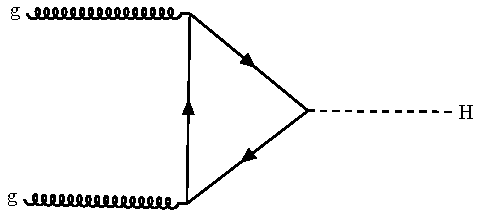
\includegraphics{../Pictures/generate_feynman_higgs/higgs-feynman.pdf}
  \captionof{figure}{Erzeugung eines Higgs-Bosons aus zwei Gluonen über eine Fermionenschleife.}
  \label{Higgs-aus-gg}
\end{center}
In der Regel wird es sich bei den Fermionen um top-Quarks handeln, da diese die größte Masse haben und daher am stärksten an das Higgs-Feld koppeln.
Da das Higgs-Boson nur eine Lebensdauer von etwa \SI{10e-22}{\second} hat erreicht es den Detektor selbst nicht.
Nachgewiesen werden können also nur die Zerfallsprodukte des Higgs-Bosons.
Man möchte hierbei natürlich Kanäle mit möglichst hohem Wirkungsquerschnitt betrachten.
In diesem Versuch wollen wir den Zerfall in zwei W-Bosonen untersuchen.
\begin{center}
  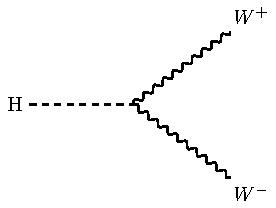
\includegraphics{../Pictures/generate_feynman_HWW/HWW-feynman.pdf}
  \captionof{figure}{Zerfall eines Higgs-Bosons in zwei W-Bosonen.}
  \label{HWW}
\end{center}
Die W-Bosonen erreichen den Detektor jedoch auch nicht selbst und zerfallen weiter.
\begin{center}
  \begin{minipage}[t]{0.45\textwidth}
    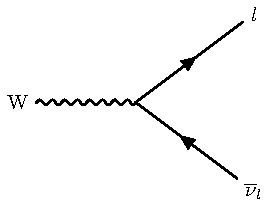
\includegraphics{../Pictures/generate_feynman_Wlnu/Wlnu-feynman.pdf}
    \captionof{figure}{Zerfall eines W-Bosons in ein Lepton und ein Lepton-Neutrino}
		\label{Wlnu}
  \end{minipage} \quad
  \begin{minipage}[t]{0.45\textwidth}
    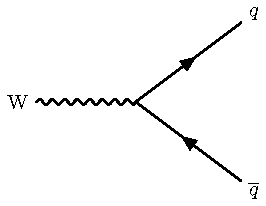
\includegraphics{../Pictures/generate_feynman_Wqq/Wqq-feynman.pdf}
    \captionof{figure}{Zerfall eines W-Bosons in Quark und Antiquark Paar.}
		\label{Wqq}
  \end{minipage}
\end{center}
Dabei können beide Bosonen unabhängig voneinander zerfallen, es gibt also drei mögliche Endzustände:
\begin{itemize}
  \item 4 Quarks (\glqq hadronischer Zerfall\grqq{})
  \item 2 Quarks, 1 Lepton und 1 Lepton-Neutrino (\glqq semileptonischer Zerfall\grqq{})
  \item 2 Leptonen und 2 Lepton-Neutronos (\glqq leptonischer Zerfall\grqq{})
\end{itemize}
Die Neutrinos können jedoch wie bereits erwähnt nicht im Detektor nachgewiesen werden und treten nur als fehlender Transversalimpuls auf.
Da Quarks zu Jets clustern ist deren Auswertung schwieriger.
Wir werden uns daher nur auf den leptonischen Zerfall beschränken.
Dieser kann wiederrum aufgespalten werden in einen Elektron-Elektron-Kanal, einen Elektron-Myon-Kanal und einen Myon-Myon-Kanal.
(Tauonen können zwar auch entstehen, zerfallen aber selbst wieder, weshalb wir sie hier weglassen.)
Dabei ist immer ein Lepton positiv und eines negativ geladen.

Weiterhin müssen wir uns Untergrundprozesse ansehen, die später aussortiert werden müssen.
Ein wichtiger Untergrundprozess ist der Zerfall eines Z-Bosons in zwei Leptonen.
\begin{center}
  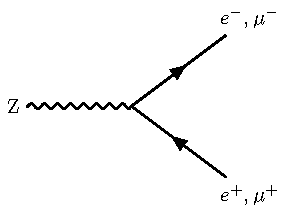
\includegraphics{../Pictures/generate_feynman_Zll/Zll-feynman.pdf}
  \captionof{figure}{Zerfall eines Z-Bosons in zwei Leptonen}
  \label{Zll}
\end{center}
Bei diesem Prozess fehlt offenbar kein Transversalimpuls, was es ermöglicht diesen Prozess von dem gesuchten zu unterscheiden.
(Oft wird der fehlende Transversalimpuls insgesamt jedoch auch bei diesem Prozess von $0$ verschieden sein. Er wird dafür relativ klein sein.)
Ein weiterer Untergrundprozess ist der Zerfall von zwei W-Bosonen die nicht aus dem Zerfall eines Higgs-Bosons entspringen.
Bei diesem liegt aber die transversal invariante Masse etwa bei der doppelten W-Masse (\SI{80}{\giga\electronvolt}).
Da das Higgs-Boson nur eine Masse von \SI{125}{\giga\electronvolt} ist bei dem gesuchten Prozess mindestens eines der W-Bosonen off-shell. (Es folgt also nicht der relativistischen Energie-Impuls-Beziehung $E^{2} = p^{2}c^{2} + m^{2}c^{4}$.)
Die invariante Masse der beiden W-Bosonen liegt dann etwa bei der Higgs-Masse.

\subsection{Das $Z'$-Boson}
Das $Z'$-Boson ist ein hypothetisches Teilchen welches als Erweiterung des Standardmodells postuliert wurde.
Seine mögliche Existenz wird dabei mit der Erweiterung der elektroschwachen Symmetrie begründet.
Dabei gibt es verschiedene Modelle mit denen das Standardmodell erweitert werden könnte.
Natürlich müsste man dafür das Teilchen jedoch ersteinmal nachweisen.
Das $Z'$-Boson wird postuliert als ein neutrales, massebehaftetes Teilchen mit Spin $1$.
Es taucht beispielsweise in Theorien der großen Vereinheitlichung (GUT) und in supersymmetrischen Theorien (SUSY) auf.
Der Massenbereich des Teilchens reicht je nach Theorie von der elektroschwachen Skala bis zur Planck-Skala.
Die Produktion des $Z'$-Bosons am LHC würde, ähnlich wie beim Z-Boson, über die Annihilation eines Quark-Antiquark-Paares geschehen.
Aufgrund der höheren Masse ist jedoch auch der Wirkungsquerschnitt bei der Produktion des $Z'$-Bosons geringer als der des Z-Bosons.
Es entstehen folglich deutlich weniger $Z'$-Bosonen.
Auch der Zerfall des $Z'$-Bosons sieht etwas anders aus.
Wegen der höheren Masse koppelt es an alle Fermionen, sodass der Zerfall in alle Kanäle des Z-Bosons und in ein $t\overline{t}$-Paar möglich ist.
Un diesem Versuch wird der Zerfall in ein $t\overline{t}$-Paar untersucht.

\subsection{Statistik}
\subsubsection{Wahrscheinlichkeitsdichte}
Eine wichtiges Werkzeug in der Statistik ist die Wahrscheinlichkeitsdichtefunktion (PDF).
Sie wird verwendet um kontinuierlich verteilte Zufallsvariablen zu beschreiben.
Dabei kann sie für eine solche Zufallsvariable $\xi$ wie folgt definiert werden:
\begin{gather}
	f(x) = \frac{dP\left (x\leq \xi <x+dx\right )}{dx}
\end{gather}
Wobei $P\left (x\leq \xi <x+dx\right )$ die Wahrscheinlichkeit darstellt, dass $\xi$ zwischen $x$ und $x+dx$ liegt.
Die PDF folgt folgenden Axiomen:
\begin{gather}
	f(x) \geq 0 \quad \forall	x \in E \\
	\int_{E} f(x)dx = 1 \\
	f(A \cup B) = f(A) + f(B) \quad \forall A,B \subseteq E, A \cap B = \emptyset
\end{gather}

Die PDF kann neben Zufallsvariablen auch weitere, feste Parameter haben.
Wir schreiben im Folgenden dafür die PDF in der Form
\begin{gather}
	f = f(x_{1},...,x_{N}|\mu_{1},...,\mu_{M})
\end{gather}
Sie beschreibt die Wahrscheinlichkeit die Ereignisse $x_{1},...,x_{N}$ zu messen, wenn für die Verteilung die Parameter $\mu_{1},...,\mu_{M}$ angenommen werden.

\subsubsection{Likelihood-Funktion}
In den meisten Experimenten ist wenigstens einer der Parameter $\mu_{i}$ unbekannt.
Man sucht dann den sogenannten \glqq besten Schätzer\grqq{}, also den Wert für die gesuchten Parameter, mit dem die PDF die beobachteten Wahrscheinlichkeiten der Ereignisse am besten beschreibt.
Diese besten Schätzer kann man mithilfe der Likelihood-Funktion finden.
Sie ist definiert als
\begin{gather}
	l(\mu_{1},...,\mu_{M}) = c \cdot \prod_{i=1}^{N} f_{i}(x_{i}|\mu_{1},...,\mu_{M})
\end{gather}
Dabei ist $c$ eine Normierungskonstante und die $f_{i}(x_{i}|\mu_{1},...,\mu_{M})$ sind die Marginalverteilungen.
Die besten Schätzer $\hat{\mu}_{1},...,\hat{\mu}_{M}$ sind dann gefunden, wenn $l$ maximal wird.
Geht man davon aus, dass die Messwerte nur von einem Parameter abhängen, kann man den besten Schätzer also einfach ermitteln mit
\begin{gather}
	\left. \frac{dl}{dp} \right |_{\hat{\mu}} = 0
\end{gather}
Oft wird statt der Likelihood-Funktion die Log-Likelihood-Funktion verwendet, welche definiert ist als
\begin{gather}
	L(\mu_{1},...,\mu_{M}) = \ln{l(\mu_{1},...,\mu_{M})} = \sum_{i=1}^{N} \ln{f_{i}(x_{i}|\mu_{1},...,\mu_{M})}
\end{gather}
Aufgrund der strengen Monotonie des Logarithmus ist diese Funktion für den selben Schätzer maximal.

\subsubsection{p-Value}
Der p-Value ist im gewissen Sinne ein Maß dafür, wie gut eine Theorie die Ergebnisse einer Messung beschreibt.
Diese Theorie wird als Nullhypothese bezeichnet.
Den p-Value kann man daher auch benutzen um eine bisherige Theorie zu überprüfen und gegebenenfalls zu falsifizieren.
Eine Theorie wird in der Regel dann verworfen, wenn der p-Value kleiner als $\num{0.05} \ (\text{entspricht} \ 2 \sigma)$ ist.
Von neuer Physik spricht man typischerweise bei einem p-Value von unter $\num{5.7e-7} \ (\text{entspricht}\  5 \sigma)$.
\begin{figure}
	\centering
  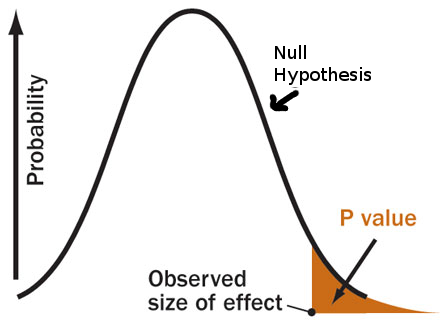
\includegraphics[width=0.85\textwidth]{../Pictures/p_value.png}
  \caption{Grafische Darstellung des p-Value \cite{p_val}}
  \label{fig_p_value}
\end{figure}
Aus Abbildung \ref{fig_p_value} geht hervor, dass der p-Value berechnet werden kann, indem man die Nullhypothese von einem bestimmten Wert an integriert.
Dieser Wert wird bestimmt mithilfe der sogenannten Teststatistik, die sich aus vielen Messwerten einer Messung ermitteln lässt.
Für diesen Versuch ist sie wie folgt definiert
\begin{gather}
	t_{\mu} = -2 \ln{\frac{\mu}{\hat{\mu}}}
\end{gather}
wobei $l(\mu)$ die Likelihood-Funktion und $l(\hat{\mu})$ die Likelihood-Funktion des besten Schätzers ist.
Der p-Value kann dann über folgende Formel berechnet werden
\begin{gather}
	p = \int_{t_{\mu}}^{\infty} f(t_{\mu}|\mu)dt_{\mu}
\end{gather}

\textbf{Anwendung auf die Teilchensuche}

Bei der Suche nach einem Teilchen geht man stets davon aus, dass das bekannte Modell stimmt, es stellt unsere Nullhypothese dar.
Mithilfe von Monte-Carlo-Simulationen kann man mit diesem Modell berechnen, wie das Ergebnis einer bestimmten Analyse erwartet wird.
Diese Vorhersage wird jetzt als Untergrund $b$ verwendet.
Ein neues Teilchen kann auch mithilfe von Modellen beschrieben werden, und es können ebenfalls Monte-Carlo-Simulationen durchgeführt werden.
Die daraus für das Teilchen gewonnene Vorhersage wird als Signal $s$ benannt.
Diese Vorhersage wird dann mit der Messung $n$ verglichen.
Existiert das Teilchen wie postuliert, dann sollten in der Messung $b+s$ Ereignisse in allen Bins eines Histogramms sein.
Als Parameter für unsere PDF wählen wir also die Signalstärke $\mu$.
Diese ist immer größer als $0$ und in der Regel kleiner als $1$.
Wir gehen nun davon aus, dass die Messwerte in den einzelnen Bins poissonverteilt sind.
Damit ergibt sich für jeden Bin die PDF
\begin{gather}
	g_{i}(n_{i}|\mu) = \frac{\left ( \mu s_{i}+b_{i}\right)^{n_{i}}}{n_{i}!} e^{-\left ( \mu s_{i}+b_{i}\right)}
\end{gather}
Die Likelihood-Funktion ist dann das Produkt über alle Bins
\begin{gather}
	l(\mu) = \prod_{i=1}^{N} \frac{\left ( \mu s_{i}+b_{i}\right)^{n_{i}}}{n_{i}!} e^{-\left ( \mu s_{i}+b_{i}\right)}
\end{gather}
Die Teststatistik wird noch ein wenig angepasst.
Da es keinen Sinn macht eine Signalstärke von weniger als $0$ zu haben wird der beste Schätzer für diesen Fall einfach zu $\hat{\mu} = 0$ gesetzt. Damit ergibt sich für die Teststatistik
\begin{gather}
	\tilde{t}_{\mu} = -2\ln{}
	\begin{cases}
  	\frac{l(\mu)}{l(\hat{\mu})}, & \hat{\mu} \geq 0 \\
    \frac{l(\mu)}{l(0)}, & \hat{\mu} < 0
  \end{cases}
\end{gather}
Möchte man den p-Value für $\mu = 0$, also für die Nullhypothese berechnen, so vereinfacht sich die Teststatistik zu
\begin{gather}
	\tilde{t}_{0} =
	\begin{cases}
		-2 \ln{\frac{l(0)}{l(\hat{\mu})}}, & \hat{\mu} \geq 0 \\
		0, & \hat{\mu} < 0
	\end{cases}
\end{gather}
Und der p-Value für die Nullhypothese ergibt sich zu
\begin{gather}
	p_{0} = \int_{\tilde{t}_{0}}^{\infty} f(\tilde{t}_{0} | \mu = 0) d\tilde{t}_{0}
\end{gather}
Für die Berechnung des p-Value fehlt aber noch die PDF der Nullhypothese.
Diese wird aus Pseudo-Daten generiert.
Man geht dafür davon aus, dass die Nullhypothese wahr ist ($\mu = 0$) und das die Messwerte in den Bins poissonverteilt sind.
Damit ergibt sich die PDF in den Bins
\begin{gather}
	g_{i}(n_{i} | \mu = 0) = \frac{b_{i}^{n_{i}}}{n_{i}!} e^{-b_{i}}
\end{gather}
mit welcher Pseudo-Daten erstellt werden können.
Mit diesen Pseudo-Daten kann dann die Teststatistik $t_{0}$ berechnet werden, mehrere $1000$ mal.
Da wir dann eine diskrete Verteilung der Teststatistik haben müssen wir für den p-Value nicht integrieren sondern summieren
\begin{gather}
	p_{0} = \sum_{t_{0} > \tilde{t}_{0}} f(t_{0}|\mu = 0)
\end{gather}

\subsubsection{obere Grenze für die Signalstärke}
Der p-Value gibt aufschluss darüber, ob die gemessenen Daten mit der Nullhypothese beschrieben werden können oder nicht.
Er sagt aber nicht direkt aus, dass unser Signal die Ursache dafür ist.
Man kann jedoch auch eine obere Grenze für die Signalstärke $\mu$ angeben.
Dafür führt man eine neue Teststatistik ein
\begin{gather}
	q_{\mu} =
	\begin{cases}
		-2 \ln{\frac{l(\mu)}{l(\hat{\mu})}}, & \hat{\mu} \geq 0 \\
		0, & \hat{\mu} < 0
	\end{cases}
\end{gather}
Man kann dann nach dem selben Prinzip oben den p-Value berechnen.
Es wird also zunächst ein $\tilde{q}_{\mu}$ aus echten Daten ermittelt, dann weitere $q_{\mu}$ aus Pseudo-Daten.
Der p-Value wird dann berechnet durch
\begin{gather}
	p_{\mu} = \sum_{q_{\mu} > \tilde{q}_{\mu}} f(q_{\mu}|\mu)
\end{gather}
Dieser p-Value wird berechnet für viele $\mu > \hat{\mu}$, und das $\mu$ bei dem der p-Value das erste mal unter \num{0.05} fällt, ist die obere Grenze.

\subsubsection{Cuts und Signifikanz}
Cuts sind ein wichtiges Werkzeug um Untergrundprozesse zu ignorieren.
Da einige Wechselwirkungen viel unwahrscheinlicher sind als andere kann es passieren, dass ein untersuchter Prozess, wie beispielsweise die Produktion eines Higgs-Bosons, sehr viel seltener passiert als ein Konkurrenzprozess, in diesem Beispiel die Produktion eines Z-Bosons.
Dadurch sind seltene Prozesse in den Daten als ganzes quasi nicht zu beobachten.
Abhilfe schaffen dabei Cuts.
Sie beschreiben das filtern der genutzten Ereignisse.
Man kann dabei nach ganz verschiedenen Kriterien filtern.
Man könnte zum Beispiel nur Ereignisse ansehen, in deren Endzustand nur ein Lepton entsteht, oder in denen es einen großen fehlenden Transversalimpuls gibt.
Das würde einige Z-Boson-Ereignisse aussortieren, da bei deren Zerfall zwei gut detektierbare Leptonen entstehen.
Dies wird aber nicht alle ungewollten Ereignisse aussortieren, da es weitere Nebenprozesse geben kann, die zu weiteren Teilchen im Endzustand führen können, und da es auch Detektorfehler gibt.
Daher schneiden Cuts auch immer einige Ereignisse unseres Signals heraus.
Es gilt also Cuts zu finden, die sehr viel mehr Untergrund als Signal entfernen.
Ein Maß für die Güte der Cuts ist die Signifikanz.
Diese ist für diesen Versuch gegeben durch
\begin{gather}
	s =
	\begin{cases}
		\sqrt{2 \cdot [(s+b) \cdot \ln{(1+\frac{s}{b})} - s]}, & \hat{\mu} \geq 0 \\
		0, & \hat{\mu} < 0
	\end{cases}
\end{gather}
wobei $s$ bzw. $b$ für die Gesamtanzahl der Signal- bzw. Untergrundereignisse steht, die nach Anwenden der Cuts noch in die Auswertung mit einfließen.
Für eine große Anzahl an Untergrundereignissen kann diese angenähert werden mit
\begin{gather}
s =
\begin{cases}
	\frac{s}{\sqrt{b}}, & \hat{\mu} \geq 0 \\
	0, & \hat{\mu} < 0
\end{cases}
\end{gather}
